\newpage
\section{Architettura dei Processori moderni}
La classica architettura di un processore, sull'esecuzione delle istruzioni, è poco efficiente, poichè bisogna aspettare sempre il termine di un istruzione per eseguire quella successiva.
Per velocizzare tale tipologia di sistema abbiamo 2 principali strade:
\begin{itemize}
    \item \textbf{Elettronicamente}: Quindi andiamo ad aumentare la frequenza di clock all'interno del nostro sistema (in gergo si utilizza il termine Overcloccare). Tale soluzione, per quanto semplice, è molto pericolosa, poichè dopo una certa soglia, non posso più aumentare la frequenza di clock. Aumentare troppo il clock potrebbe far danneggiare i componenti per la troppa energia da dissipare e quindi bisognerebbe prevedere anche delle architetture costruite ad-hoc
    
    \item \textbf{Architetturalmente}: Vado a modificare l'architettura per gestire un nuovo modo di funzionamento del classico flusso di funzionamento di un processore. Tale modifica permetterebbe di poter eseguire più istruzioni contemporaneamente. Le tipologie di approcci che si possono avere in base a questa soluzione sono 2:
    \begin{itemize}
        \item \textbf{Parallelismo livello di Processo}: Ho a disposizione più processori (parallelismo esplicito) che vanno ad eseguire in maniera concorrente tali processi
        \item \textbf{Parallalismo livello istruzione}: Un singolo processore riesce ad eseguire più istruzioni in maniera parallela
    \end{itemize}
\end{itemize}

Le due macrosoluzioni non sono mutuamente esclusive, quindi si potrebbe anche pensare di effettuare una combinazione di esse.
Guardando nello specifico alla soluzione di tipo \textbf{Architetturale} si possono incontrare varie strade per poter implementare il parallelismo delle istruzioni.
Per poter meglio comprendere come effettuare la suddivisione del lavoro tramite le varie architetture, bisogna comprendere bene come strutturare un \textbf{Processo}. Tale entità la possiamo vedere come:
\begin{itemize}
    \item Formata da più task disgiunti ed indipendenti
    \item Formata da un solo programma che richiede un'esecuzione ad elevate prestazioni
\end{itemize}

Le architetture che negli anni sono state progettate per la distribuzione del carico di lavoro, dato da un singolo processo sono varie (quindi ci troviamo nel secondo caso).
Le tipologie principali sono:
\begin{itemize}
    \item \textbf{SISD (Single Istruction Single Data)}: Architettura in grado di eseguire una istruzione alla volta lavorando su dati singoli. Tale tipologia di architettura rispetta per filo e per segno la classica architettura di Von Neumann, la tipologia di parallelismo che si può implementare su tali sistemi è solo tramite un cambio di contesto, quindi definendo uno scheduling.
    \item \textbf{SIMD (Single Istruction Multiple Data)}: Architettura progettata per l'esecuzione di una singola istruzione su più dati. Tale tipologia di architettura è molto buona per l'esecuzione di prodotti vettoriali. Il parallelismo di tale macchina è intrinseco rispetto ai dati, poichè si agisce effettuando una singola istruzione sui vari dati
    \item \textbf{MISD (Multiple Istruction Single Data)}: (Tali architetture sono state aggiunte solo per conoscenza personale, ma non sono state spiegate dal professore) Architettura in grado di eseguire una moltitudine di istruzioni su di un singolo dato. Tale tipologia di architettura è la meno utilizzata, poichè si cerca di eseguire sempre delle operazioni contemporanee rispetto ai dati
    \item \textbf{MIMD (Multiple Istruction Multiple Data)}: Architettura che consente di eseguire più istruzioni su più dati. Essi eseguono quindi in parallelo, più istruzioni diverse su più dati diversi. Esse sono le più complicate per via della condivisione della memoria, difatti, ve ne sono varie, in base a come si vadano ad accedere i vari dati in memoria
\end{itemize}

Nel nostro caso, il Motorola 68k è una tipologia di sistema \textbf{SISD}.
Ad oggi i sistemi maggiormente utilizzati sono i sistemi \textbf{MIMD}, che prevedono l'utilizzo di più unità di elaborazione per poter determinare uno specifico risultato. Tali sistemi, come detto in precedenza, possono essere di vario tipo e possono essere strutturati in vario modo.
Un primo approccio è quello di costruire due sistemi "gemelli", ovvero, costruire due calcolatori differenti che tramite la comunicazione I/O gestiscono le varie operazioni da effettuare. Tale sistema, però, non è molto efficente, poichè le comunicazioni tramite dispositivi di I/O non è veloce come i processori, per cui si avrebbe un rallentamento delle operazioni.
Per sopperire a tale problema, allora si potrebbe pensare di utilizzare un sistema di memoria condivisa tra i due processori, in modo da evitare i dispositivi di I/O. La problematica che si andrebbe a presentare in quest'altro caso sarebbe l'accesso al BUS, che nonostante sia velocissimo, ha bisogno di una buona comunicazione tra i due processori.
Per migliorare ancora tale tipologia di architettura, allora, si potrebbe pensare di utilizzare una gerarchia di memorie, che permetta di ridurre gli accessi in memoria pilotati dai vari processori, che possono lavorare sulle loro memoria "private" in maniera del tutto autonoma e concorrente senza dover schedulare l'accesso al BUS.

\begin{figure}
    \centering
    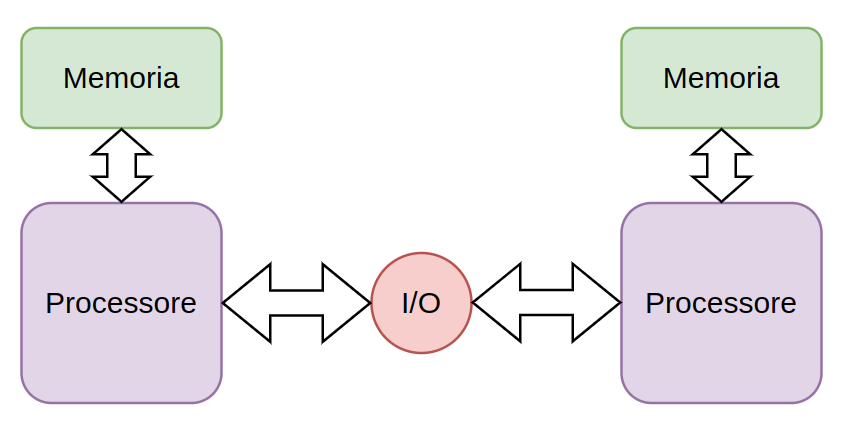
\includegraphics[width=.5\textwidth]{img/P-IO-P.png}
    \caption{Sistemi "gemelli" o sistema multicomputer}\label{img:multi-computer}
\end{figure}

\begin{figure}
    \centering
    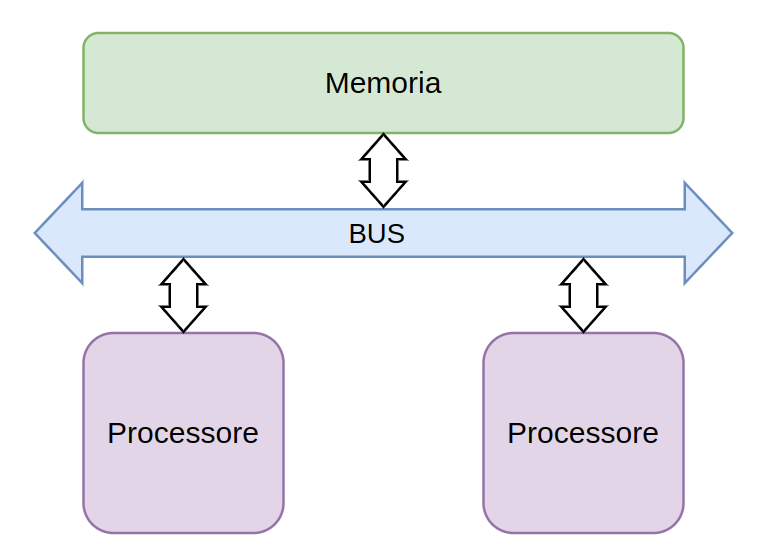
\includegraphics[width=.5\textwidth]{img/P-BUS-P.png}
    \caption{Sistema a memoria condivisa}\label{img:shared-memory}
\end{figure}

\begin{figure}
    \centering
    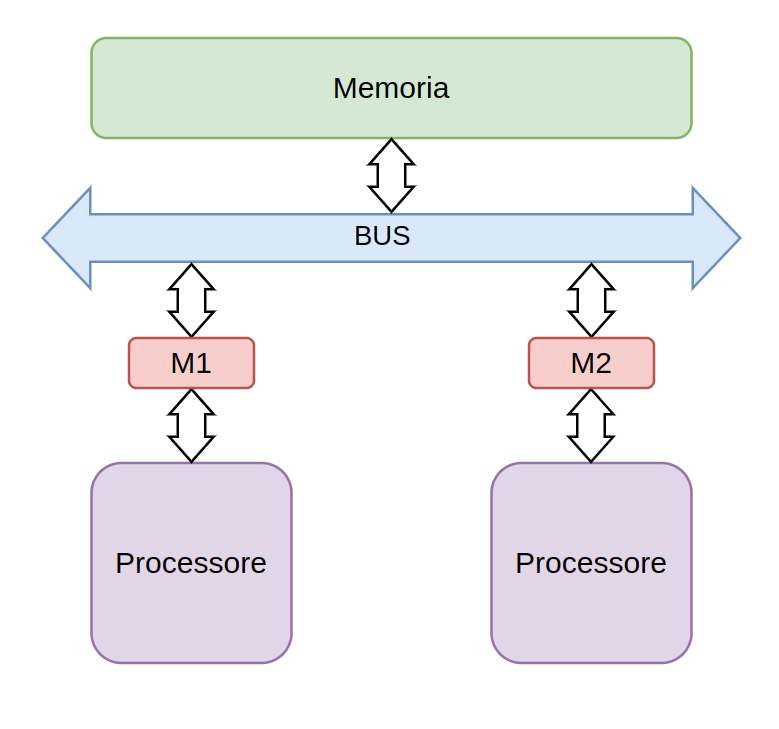
\includegraphics[width=.5\textwidth]{img/P-M-BUS-M-P.png}
    \caption{Sistema multicore}\label{img:multi-core}
\end{figure}

I sistemi che sfruttano le gerarchie di memoria prendono il nome di \textbf{sistemi multicore}, che non hanno solo 2 livelli di gerarchia di memoria, ma ne hanno vari, in base ai casi.

\newpage
\subsection{Multi-Computer e Multi-Processore}
Concentriamo la nostra attenzione sui sistemi MIMD. Escludendo la possibilità di avere un parallelismo interno, è possibile individuare due categorie di sistemi che permettono a più processori di lavorare su dati diversi, questi sono detti Multi-Computer e Multi-Processore.
\\
Un primo metodo utile a far interagire due (o più) sistemi differenti è introdurre un intermediario, ovvero un particolare tipo di sistema di I/O che sia efficace e veloce. In tal caso, quanto più rapidamente saranno i processori, tanto più dovrà essere il sistema (oltre che la rete che li interconnette). La limitazione principale di tale modello è la sensibilità ai limiti tecnologici dovuto all'interconnessione. Il sistema globale è detto \textbf{Multi-Computer} ed è particolarmente utilizzato per applicazioni che richiedono calcoli dedicati [\ref{fig:multi-computer}].
\begin{figure}[!h]
    \centering
    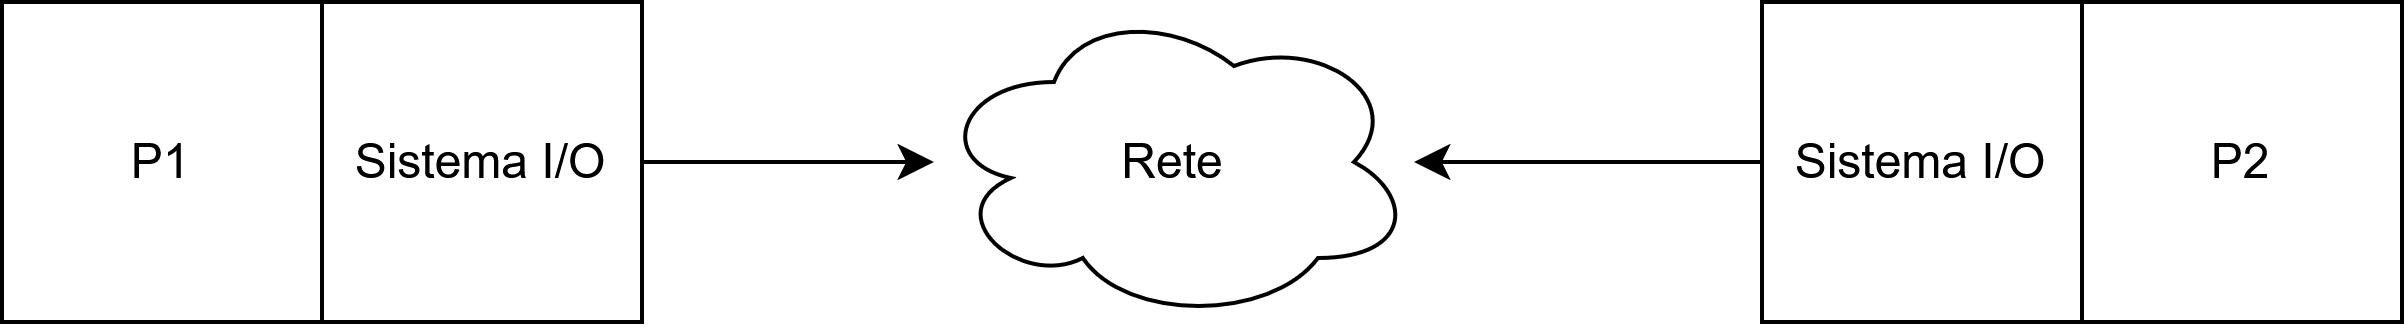
\includegraphics[width=0.8\linewidth]{img/multi-processore.png}
    \caption{Architettura di un sistema Multi-Computer.}
    \label{fig:multi-computer}
\end{figure}

Un'altra possibilità per far interagire i processori è direttamente tramite la memoria, ottenendo un sistema complessivo detto \textbf{Multi-Processore} [\ref{fig:multi-processore}]. In tal caso, la comunicazione tra i processori avviene direttamente tramite bus, superando il problema legato alla fisica realizzabilità di connessioni su larga scala. Il vantaggio di questi sistemi è che i dati possono essere trasferiti molto rapidamente in memoria grazie al bus, mentre lo svantaggio è relativo alla competizione tra i processori negli accessi in memoria. Una possibile miglioria all'architettura proposta consiste nell'integrare a ciascun processore una memoria interna più piccola che gli permetta di gestire le istruzioni. In altre parole, è necessario gestire una gerarchia delle memoria. 
Potremmo (erroneamente) pensare che aggiungere più core permetta di velocizzare il sistema, in realtà questo è sbagliato perché complicherebbe notevolmente le connessioni del bus, il quale diventerebbe il collo di bottiglia del modello.
\begin{figure}[!h]
    \centering
    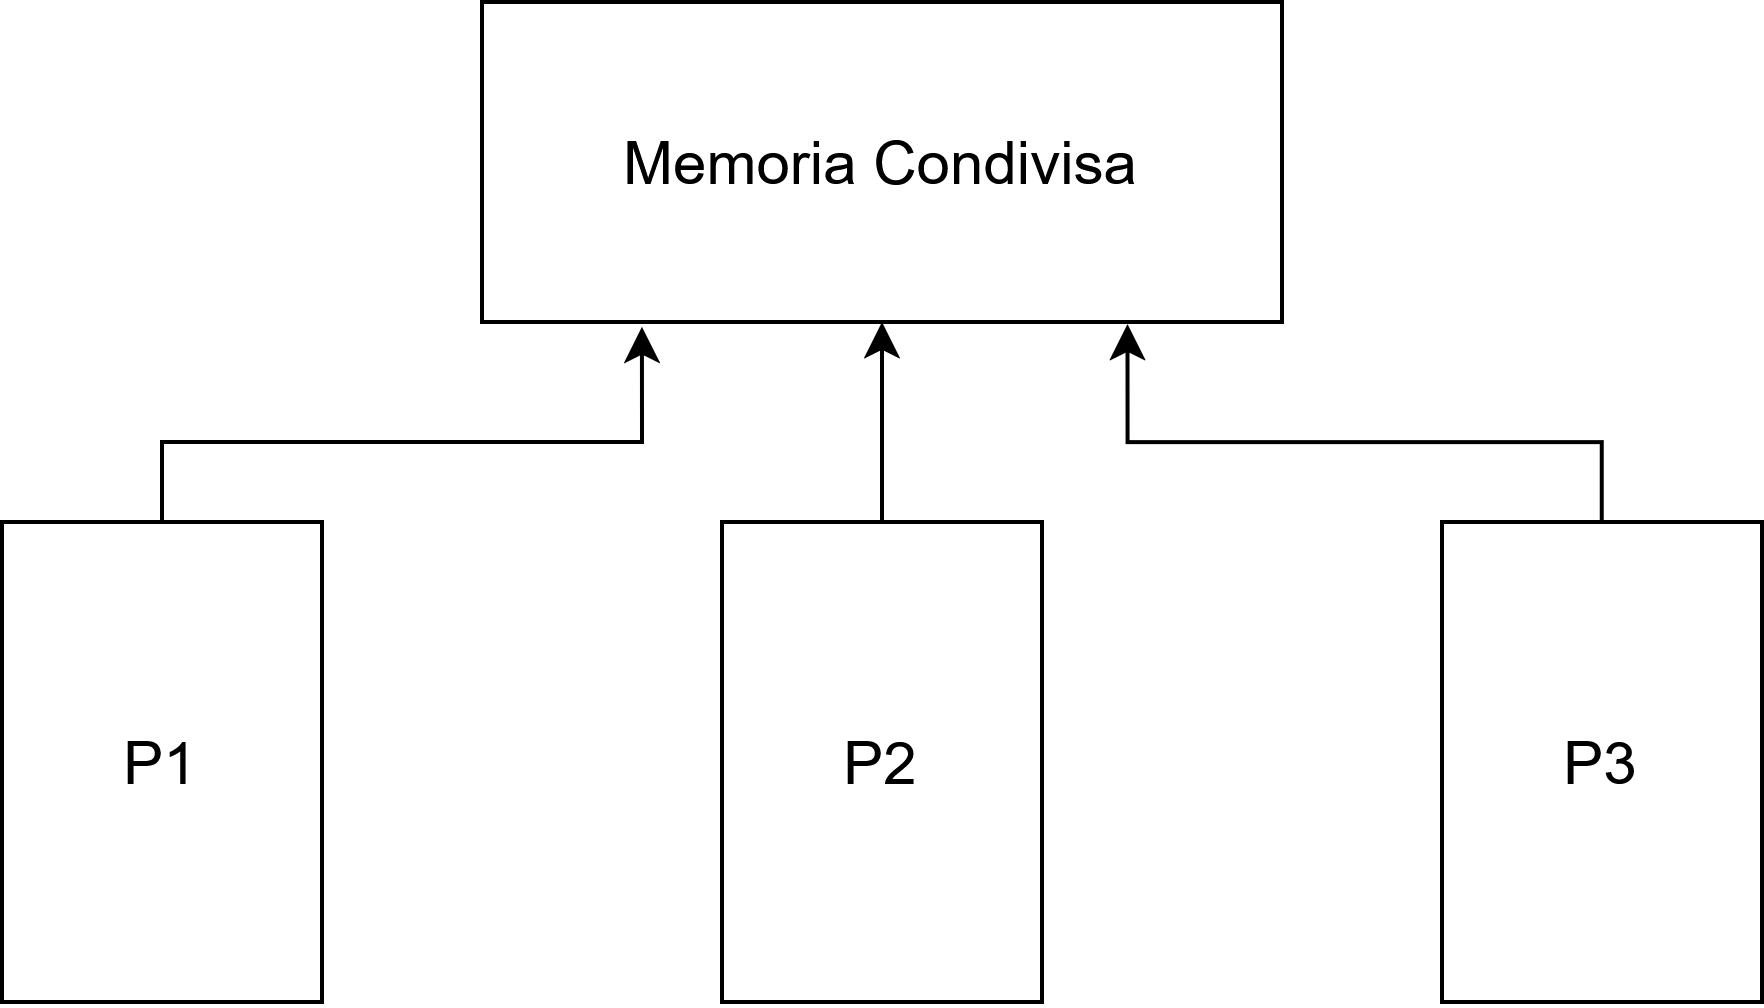
\includegraphics[width=0.5\linewidth]{img/multi-computer.png}
    \caption{Architettura di un sistema Multi-Processore.}
    \label{fig:multi-processore}
\end{figure}
L'esistenza di un modello non esclude la possibilità di inserirne un altro, cosa che accade tipicamente nei sistemi moderni.

